%______________________________________________________________________________
%************************* HEADER *********************************************
\documentclass[]{scrreprt}
		
    
\usepackage{a4}
\usepackage[T1]{fontenc}
\usepackage[utf8]{inputenc}
\usepackage{lmodern}

\usepackage{subfigure}
\usepackage{epsfig}
\usepackage{graphicx}
\usepackage{graphics}
% \usepackage{array}
% \usepackage{units}
%\usepackage{cite}	 % Für Bibtex
\usepackage[noadjust]{cite}	 % Für Bibtex, noadjust: Keine Leerzeichen vor Referenz _[X]
\usepackage[]{placeins}  % für \FloatBarrier
\usepackage{amssymb} 
\usepackage[]{amsmath}   % Formelumgebung für begin{align]
% \usepackage{longtable}   % Mehrseitige Tabellen (Symbole)
\usepackage{booktabs}    % horizontale Linien in Tabellen
\usepackage{wrapfig}
% \usepackage{listings}    % Für Quellcode einbinden
\usepackage[onehalfspacing]{setspace}   % Einfacher Zeilenabstand für Tabellen
\usepackage{tabularx}

% \usepackage{tocbasic}
\usepackage[pdfpagelabels, plainpages=false]{hyperref} 
% \usepackage[linktocpage,pdfborderstyle={/S/U/W 1}]{hyperref}  % Links nur unterstrichen, nicht umrandet




% ---------------- header ----------------------
\usepackage{scrlayer-scrpage}
\automark{chapter}
\automark*{section}
\clearpairofpagestyles
\ihead{\headmark}
\ohead{\pagemark}

% ---------------- Sonstige Formatierung ----------------------
% \setlength{\parindent}{6pt} \linespread{1.3}  % Einrücken nach Absatz,  Zeilenabstand


% ---------------- Seiten-Einstellungen ----------------------
\usepackage{geometry}
\geometry{a4paper, top=25mm, left=35mm, right=25mm, bottom=25mm,
headsep=10mm, footskip=12mm}

\usepackage{blindtext}

\title{SWAT-EM}
\subtitle{Specific Winding Analyse Tool for Electrical Machines}
\author{Martin Baun}
\date{\today}

%************************* Titelseite *****************************************
\begin{document}

\maketitle{}


%************************* Vorwort *********************************


%************************* Inhaltsverzeichnis *********************************
% Überschriften bis zur 4. Ebene nummerieren
\setcounter{secnumdepth}{4}

% Überschriften bis zur 4. Ebene ins Inhaltsverzeichnis aufnehmen
\setcounter{tocdepth}{4}

% \addcontentsline{toc}{chapter}{Inhaltsverzeichnis} % Eintrag im Inhaltsverzeichnis erzeugen
\tableofcontents        %Inhaltsverzeichnis einf\"{u}gen



% \include{Abkuerzung}   % Symbolverzeichnis einbinden
% \include{Symbole}   % Symbolverzeichnis einbinden



%************************* Kapitel ********************************************
% \pagenumbering{arabic}




%************************* Literaturverzeichnis *******************************
%\appendix
%\begin{appendix}

% \bibliographystyle{unsrt}
% \bibliography{Literatur_Bib}


%************************* Tabellenverzeichnis *******************************
% \listoftables


%************************* Abbildungsverzeichnis *******************************
% \listoffigures


% \include{Einleitung}

% \cite{Bianchi_star_slot_2006}




\chapter{Overview}
SWAT-EM is a software for designing and analysing of windings systems for electrical machines. Currently supported are rotating field windings (permanent-magnet motors, induction motors, synchronout reluctance motors) with any number of phases. This can be distributed full pitch winding, distributed fractional slot winding or tooth-coil winding. The design can be done by 
\begin{itemize}
 \item Generating with manual allocation of the coil sides to stator slots
 \item Defining individual number of turns for each coil
 \item Automatic winding generators
 \item Tables of possible winding systems for slot/pole combinations
\end{itemize}
% 
% 
% 
Analyzing features
\begin{itemize}
\item Calculation of the winding factor based on the voltage star of slots
\item Plot of the winding layout
\item Plot of statorampere-conductor distribution and the magnetic motoric force (MMF)
\item Plot of the slot voltage phasors
\item Plot of the winding factor
\item Max. possible number of parallel circuit connection of coils

\end{itemize}




\chapter{Installation}

\chapter{Usage}

\section{Main window}
%
SWAT-EM comes with an QT based graphical user interface (GUI). The layout of the main window consists of the
\begin{enumerate}
 \item Workspace
 \item Winding Informations
 \item Graphical analysis of the winding
\end{enumerate}


%
\begin{figure}[htpb]
    \centering
    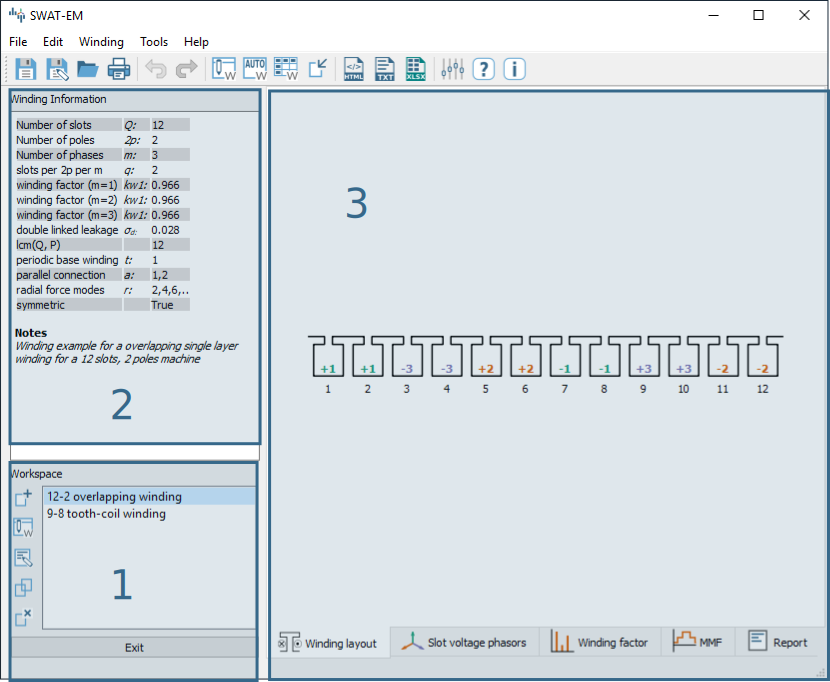
\includegraphics[width=0.99\textwidth,angle=0]{fig/mainwindow}
    \caption{Main-window}
    \label{fig:mainwindow}
\end{figure}
%
\subsection{Workspace}
A SWAT-EM project, that can be saved as *.wdg file can contain several different windings system.
So, one can define and compare these windings in the same window. The workspace shows all
the windings of the project. By clicking of the name all outputs (text and plots) gets updated.
The buttons on the left of (1) in figure \ref{fig:mainwindow} modifies the windings in the workspace
\begin{description}
 \item[New winding] Opens a dialog with all existing winding generator (see section \ref{sec:winding_generators}). 
		    One can choose any of these generators to create a winding layout.
 \item[Manual winding layout] Define the position of all coil sides by hand. (Not very comfortable
		    but full control)
 \item[Auto winding layout] Generates the winding automatically by number of slots, poles, ... (easy
                            to use, almost every symmetric winding is possible)
 \item[Winding table] Shows table slot/pole combinations (a good overview of possible combinations) 
 \item[Notes] If there a many windings in the project it might be a good idea to add some notes
              to the different layouts.
 \item[Clone] For modifying windings one can clone/duplicate an existing one. So a switch-back to the 
              initial state and a comparison is possible.
 \item[Delete] Deletes the selected winding.
\end{description}
%
While saving the project to file (File $\rightarrow$ save) all windings of the workspace are saved. 
\textbf{Note:} Renaming of windings is possible by double-click or by pressing F2 on keyboard.
%
%
\subsection{Winding information}
The text field (2) in figure \ref{fig:mainwindow} shows a summary of actual winding. 
%
\begin{center}
\begin{table}[h]
\begin{tabularx}{\textwidth}{lX}
$Q$ & Number of stator slots \\
$2p$ & Number of pole pairs  \\
$m$ & Number of phases \\
$q$ & Number of slots per pole per phase $q=\frac{Q}{2pm}$ \\
$kw1$ & Fundamental winding factor (for separate for each phase) \\
$lcm(Q,P)$ & Least common multiplyer of number of slots an pole pairs. For permanent-magnet machines this is the first harmonic  number of the cogging torque \\
$t$ & Periodicity of the base winding. $t = gcd(Q, p)$ \\
$a$ & Number of possible parallel winding circuit. (In most cases a is equal to t) \\
$symmetric$ & True, if all phases are identically and shifted by a constant angle \\
$Notes$ & User defined description \\
\end{tabularx}
\end{table}[
\end{center}


%
%
%
%
\subsection{Winding layout plot}
Many analyzing function results in plots which are shown on(3) in figure \ref{fig:mainwindow}.
Every plot has a toolbar on the bottom for zooming, panning and saving the figure to file.
%
%
\subsubsection{Winding layout}
The winding layout plot shows sketched slots and coil sides. The number and color defines the number
of phase the coil side belongs to. The sign (+ or -) defines the winding direction (+ means that the
wire goes into the plain and - out of the plain)
%
%
\subsubsection{Slot voltage phasors}
TODO: Add Theory
%
%
\subsubsection{Winding factor phasors}
TODO: Add Theory
%
%
\subsubsection{Magnetic motoric force (MMF)}
TODO: Add Theory






\section{Winding Generators}\label{sec:winding_generators}
\subsection{Manual layout}
\subsection{Automatic layout}
\subsection{Winding table}





\bibliographystyle{unsrt}
\bibliography{literature}

\end{document}







